%Documento di proprietà di Vito Stefano Birardi™
%Qui sono presenti i package più comuni che usi, ricorda di usare solo quelli che ti servono 

%Variabili comuni
\newcommand{\Titolo}{Progetto A\_Clus - Documentazione}
\newcommand{\Data}{\today}
\newcommand{\Materia}{}

%Comandi troppo lunghi da scrivere possono essere ri-operazionalizzati qui

\newcommand{\image}[3]{%
    \begin{figure}[h!]
    \centering
    \includegraphics[width = 0.5 \textwidth]{#1}
    \caption{#2}
    \label{#3}%
\end{figure}}

%Package per la formattazione del foglio

\documentclass[a4paper]{article}
\usepackage{amsmath}
\usepackage{amssymb}

%Package per la lingua dei capitoli

\usepackage[italian]{babel}

%Package per intestazione e pié di pagina

\usepackage{fancyvrb}
\usepackage{fancyhdr, lastpage}

%Package aggiuntivi 

\usepackage{cancel}
\usepackage{etoolbox}
\usepackage{xcolor}
\usepackage{subfig}
\usepackage{tikz, lmodern}
\usepackage[T1]{fontenc}
\usepackage[most]{tcolorbox}
\usepackage{graphicx}
\usepackage{hyperref}
\usepackage{parskip}
\usepackage{multicol}
\pagestyle{fancy}

%Formattazione di intestazione e pié di pagina


\lhead{\Data}
\rhead{Vito Stefano Birardi \\ Lorenzo Gelao}
\lfoot{\Materia}
\rfoot{Pagina \thepage\ di \pageref{LastPage}}
\renewcommand{\footrulewidth}{0.5pt}
\fancyfoot[C]{}
\patchcmd{\chapter}{\thispagestyle{plain}}{\thispagestyle{fancy}}{}

%Preambolo per prima pagina

\title{\Titolo}
\author{
    A cura di: 
    Vito Stefano \\ Lorenzo Gelao
}
\date{\Data}

%Inizio documento vero e proprio


\begin{document}
\maketitle
\newpage
\tableofcontents
\newpage

\section{Introduzione}

Il progetto in questione verte sull'argoemento dell'\textit{Agglomerative Clustering}, una tecnica di clusterizzazione basata sui metodi Signle distance e Average Distance. 

Il progtto in questione è suddiviso in una parte client e una server, che comunicando tra loro, generano il dendrogramma, permettendo inoltre di visualizzare e memorizzare tali risultati o di caricarne dei precedenti.

È inoltre possibile visualizzare nuovamente dei file caricati in passato per visualizzare i cluster e i dendrogrammi associati. 


\subsection{Agglomerative Clustering}

L'algoritmo di clustering utilizzato in tale progetto, come si può desumer dal nome, sfrutta il concetto di clustering agglomerativo. In pratica, tratta ciascun cluster in maneira separata dagli altri, unendo progressivamente quelli più vicini, in base a due crtieri principali, nel nostro caso.

Il princiaple vantaggio  rispetto ad altri algoritmi di lcustering, come il k-means, è che in questo modo non è necessario speficiare in anticippo la quantità di cluster da analizzare. 

I criteri utilizzati nel progetto A-CLus sono i seguenti: 

\begin{enumerate}
    \item \textbf{Single-Link}: tale criterio determina la distanza minima tra i punti dei vari cluster

    \begin{equation}
        D\left(C1,C2\right) = \underset{\left(t1 \in C1,t2 \in C2\right)}{min}\left( dist\left(t1,t2\right)\right)
    \end{equation}
\end{enumerate}


Durante l'anno accademico 2024/2025, l'oggetto di ricerca è stato incretrato su "A-CLus", una piattaforma con architettura client-server dedicata all'analisi dei dati mediante algoritmi di clustering gerarchico agglomerativo. La componente server esegue le operazioni di clustering impiegando le metodologie Single Link o Average Link per il calcolo delle distanze inter-cluster e la successiva costruzione del dendrogramma. L'applicativo client, implementato in linguaggio Java, offre agli utenti diverse funzionalità: il caricamento o la creazione di istanze HierarchicalClusterMiner, la rappresentazione grafica del dendrogramma e l'archiviazione dei risultati per analisi successive. È inoltre disponibile la funzione di importazione di file precedentemente salvati, consentendo agli utenti di riesaminare i cluster e i relativi dendrogrammi. 

\subsubsection{Framework Analitico}

La tecnica di clustering agglomerativo implementata nel sistema "A-CLus" costituisce una metodologia avanzata per l'identificazione di \underline{correlazioni latenti nei dataset}. 

Diversamente da tecniche alternative come il k-means, l'approccio agglomerativo elimina la necessità di predefinire il numero di raggruppamenti. La procedura inizializza ciascun elemento come cluster individuale e procede con l'unificazione sequenziale dei cluster con maggiore affinità, applicando metodologie quali:  



Con il procedere delle aggregazioni tra cluster, si sviluppa un dendrogramma che illustra la gerarchia delle aggregazioni. Il procedimento continua fino al raggiungimento di un cluster unificato o fino a una soglia di profondità stabilita dall'utilizzatore. La visualizzazione mediante dendrogramma rende la metodologia particolarmente comprensibile, facilitando l'esplorazione strutturale dei dati a diversi livelli di granularità. Inoltre, questa strategia non è influenzata dalla configurazione iniziale dei centroidi, riducendo così la probabilità di risultati inconsistenti e garantendo una rappresentazione più accurata dell'organizzazione interna del dataset.RiprovaClaude può commettere errori. Verifica sempre le risposte con attenzione.



\section{Guida all'installazione}

Prima di essere in grado di eseguire il programma, è necessario eseguire il file \texttt{risorse.bat} contenuto nella cartella Risorse. 


Una volta eseguito il file, si aprirà una pagina ti Powershell e seguirà un download.

\begin{figure}[h!]
    \centering
    
\includegraphics[width= 0.5\textwidth]{images/nuova docs.png}
    \caption{Schermatta di download}
\end{figure}

Al termine del download del file compresso delle risorse, verranno estratti i file necessari per l'esecuzione del programma.



Per il progetto in questione è necessario installare il Java Developer Kit (JDK) nella versione 22.0.1 e il software di gestione del database MySQL nella sua versione 8.0.39. 

La prima scheda di installazione che apparirà è quella del JDK. 

Verrà chiesto se si vuole eseguire l'installazione del JDK tramite permessi di amministratore, cliccare su \underline{Sì}.

\subsection{Installazione JDK}

Una volta confermata l'esecuzione come amministratore, si procederà all'installazione del JDK.

\begin{figure}[h!]
    \centering
    
\includegraphics[width= 0.5\textwidth]{images/installazione java.png}
\end{figure}

Cliccare su \textbf{Avanti},nuovamente \textbf{Avanti} e infine, nel caso in cui l'installazione sia andata a buon fine, si dovràò cliccare sul tasto \textbf{Chiudi}.

Una volta completata l'installazione del JDK, si procederà automaticamente con l'installazione del MySQL.

\subsection{Installazione MySQL}

Anche qui sarà necessario fornire i permessi di amministratore, cliccare dunque su \underline{Sì}.

Dopodiché si aprirà la schermata di installazione di MySQL.

\begin{figure}[h!]
    \centering
    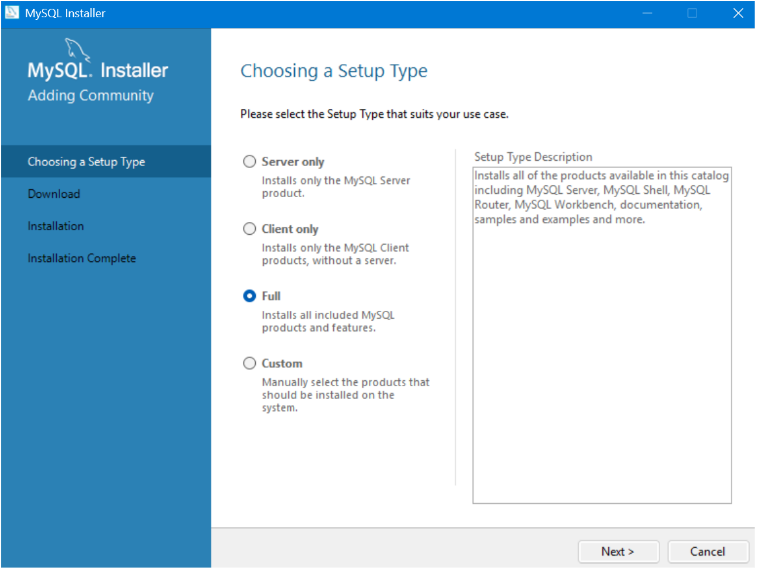
\includegraphics[width= 0.5\textwidth]{images/inizio mysql.png}
    \caption{Scelta del setup}
\end{figure}

Selezionare il tipo di setup \textbf{Full} e cliccare su \textbf{Next}. Tale scelta permetterà di installare tutti i componenti necessari per l'esecuzione del programma.

Si passerà alla schermata di download dei file necessari per l'installazione, cliccare su \textbf{Execute}. 

Tale schermata potrebbe richiedere un po' di tempo per il download dei file, a seconda della velocità della connessione internet. 

Dopo aver scaricato i file, si dovrà cliccare nuovamente su \textbf{Execute}.

\begin{figure}[h!]
    \centering
    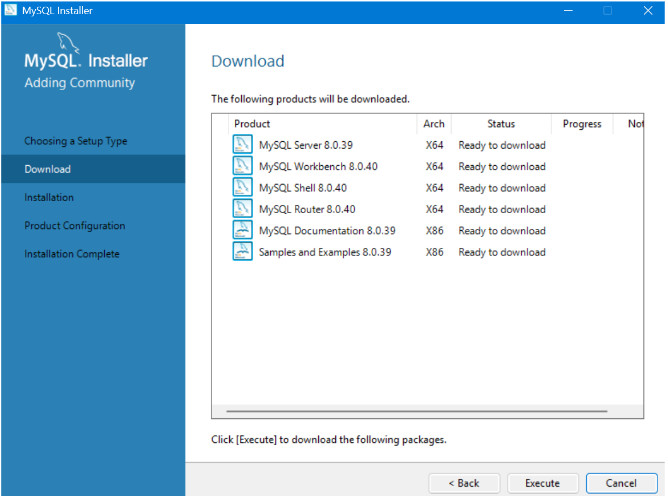
\includegraphics[width= 0.6\textwidth]{images/eexecute.png}
    \caption{Download MySQL}
\end{figure}

Una volta terminato il download, si procederà con la configurazione dell'account MySQL. Si dovrà quindi scegliere una password, necessaria per accedere al database. 


\begin{figure}[h!]
    \centering
    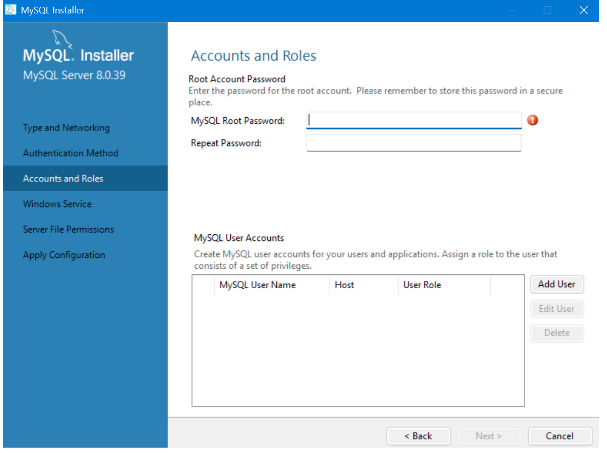
\includegraphics[width= 0.5\textwidth]{images/setup vero e proio musql.png}
    \caption{Configurazione account MySQL}
\end{figure}

Si giungerà infine alla scehermata di applicazione della configurazione del database. Cliccare su \textbf{Execute} per applicare la configurazione.

\begin{figure}[h!]
    \centering
    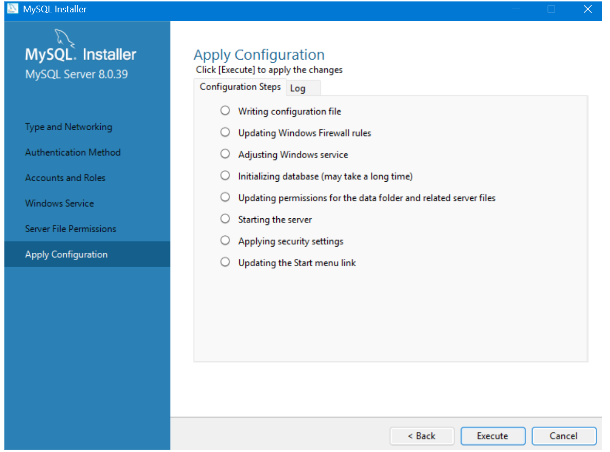
\includegraphics[width= 0.5\textwidth]{images/completamenot.png}
    \caption{Completamento installazione}
\end{figure}


\begin{figure}[h!]
    \centering
    
\includegraphics[width= 0.6\textwidth]{images/insytllazione compeltata.png}
    \caption{Completamento installazione}
\end{figure}

\section{Eseguire A-CLus Base}

\subsection{Operazioni preliminari}

Prima di poter eseguire il programma, occorre importare il database di A-CLus in MySQL. 

Tale file è presente nella cartella \texttt{A-CLus/Risorse} e si chiama \texttt{mapdb.sql}. 

Per importare il database, è necessario semplciemente accedere al MySQL tramite root e digitare il seguente comando \texttt{source} seguito dal percorso del file \texttt{mapdb.sql}. 

Tale percorso si può ottenere semplicemente trascinando il file del database sul terminale di MySQL.

Alle fine dell'importazione, il terminale di MySQL dovrebbe mostrare un messaggio simile al seguente:

\begin{figure}[h!]
    \centering
    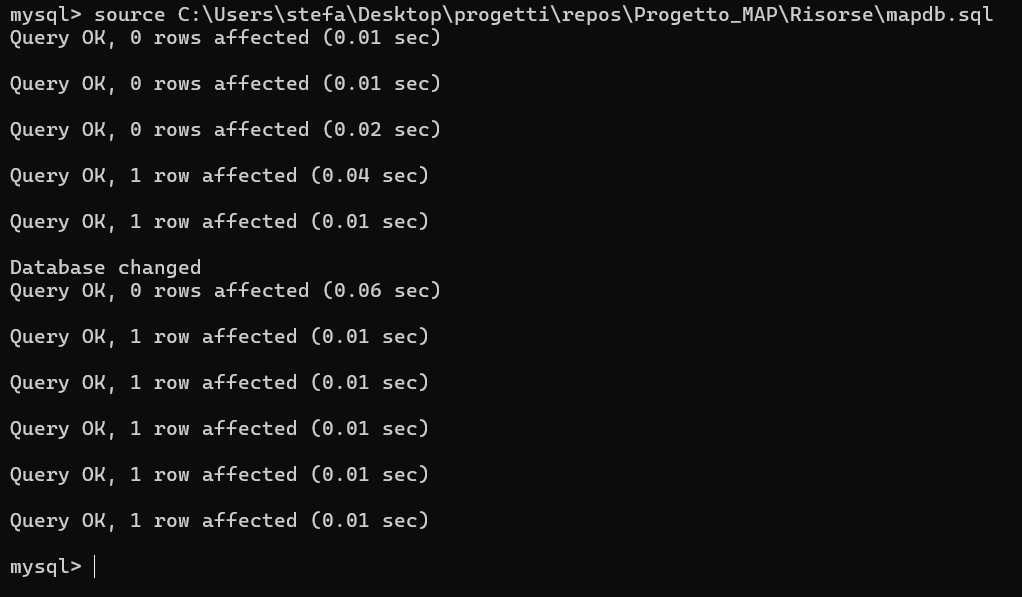
\includegraphics[width=0.5\textwidth]{images/import mysql.png}
\end{figure}

È possibile verificare la corretta importazione anche uscendo da MySQl e accedere con le credenziali dell'utente MapUser, come mostrato nella figura seguente:

\begin{figure}[h!]
    \centering
    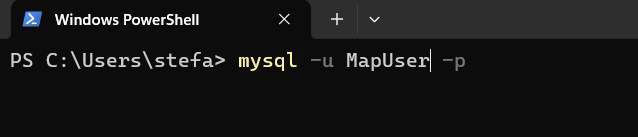
\includegraphics[width=0.5\textwidth]{images/import mapdb.png}
\end{figure}

La password dell'utente MapUser è \texttt{map}. Se viene confermato l'accesso al database, significa che l'importazione è avvenuta con successo. 

\subsection{Avvio dell'applicazione}

Per inizializzare correttamente la versione standard di A-CLus, attenersi alla seguente sequenza operativa:


\begin{enumerate}
    \item Accedere alla directory \texttt{A-CLus\_Base/Bat}
    \item Eseguire il file \texttt{Start\_Server.bat} facendo un doppio click su di esso, assicurandosi che venga mostrato il seguente messaggio a finestra
    
    \begin{figure}[h!]
        \centering
        
\includegraphics[width=0.5\textwidth]{images/server in esecuzione.png}
    \end{figure}

    \item Dopo aver verificato il corretto funzionamento del server, eseguire il file \texttt{Start\_Client.bat} facendo un doppio click su di esso; se non ci sono problemi con il server, apparirà la seguente schermata:
    
    \begin{figure}[h!]
        \centering
        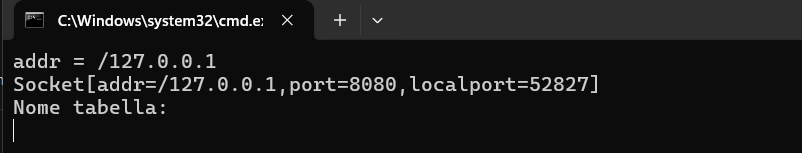
\includegraphics[width=0.5\textwidth]{images/client in esecuzione.png}
        
    \end{figure}
    
\end{enumerate}

\begin{tcolorbox}[colback=white, colframe=gray, title=Avvertenza]
    È necessario mantenere attivo il terminale del server per garantire la comunicazione tra le componenti client e server.
\end{tcolorbox}

\subsection{Avvio dell'ambiente di sviluppo}

Per aprire correttamente il codice sorgente di A-CLus, è necessario seguire le seguenti operazioni nell'ordine in cui sono presentate:

\begin{enumerate}
    \item Aprire la cartella del progetto \texttt{A-Clus\_base}
    \item Incorporare nelle librerie del progetto \texttt{Server} il file \texttt{mySQL\_connector.jar} presente nella cartella \texttt{A-CLus/Risorse}. Nel caso si stia eseguendo il progetto in Visual Studio Code, è possibile eseguire i seguenti passaggi:
    \begin{enumerate}
        \item Aprire il progetto \texttt{A-Clus\_Base}
        \item Recarsi nella sezione \texttt{Referenced Libraries}, in asso a sinistra
        \item Posizionare il cursore sulla cartella e selezionare \texttt{Add JAR/Folder Classpath}, che apparirà sulla destra
        \begin{figure}[h!]
            \centering
            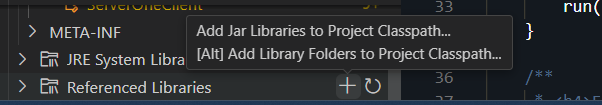
\includegraphics[width=0.5\textwidth]{images/refenereziare il jdbc.png}
        \end{figure}
    \end{enumerate}
    \item Avviare \texttt{MultiServer.java}
    \item Controllare che il server sia in esecuzione correttamente
    \item Aprire il progetto \texttt{MainTest.java} presente nella cartella \texttt{A-CLus\_Base/Client}
\end{enumerate}

\subsection{Interfaccia iniziale}

L'interfaccia iniziale di A-CLus è composta da tre sezioni principali:

\begin{figure}[h!]
    \centering
    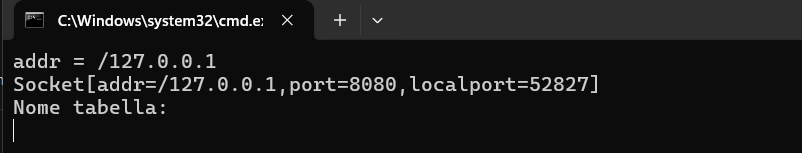
\includegraphics[width=\textwidth]{images/client in esecuzione.png}
    \caption{Interfaccia iniziale di A-CLus}
\end{figure}

L'interfaccia iniziale di A-CLus è composta da tre sezioni principali:

\begin{figure}[h!]
    \centering
    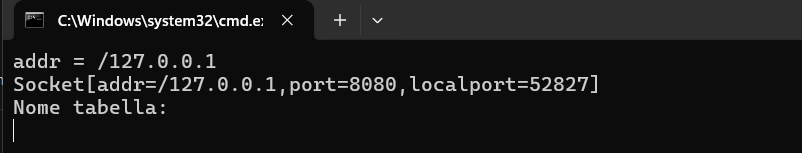
\includegraphics[width=\textwidth]{images/client in esecuzione.png}
    \caption{Interfaccia iniziale di A-CLus}
\end{figure}

\subsection{Selezione delle operazioni disponibili}

\begin{figure}[h!]
    \centering
    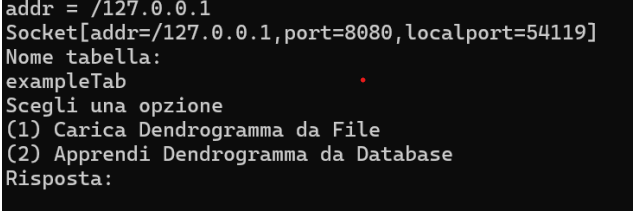
\includegraphics[width=\textwidth]{images/inserimento_tabella.png}
\end{figure}

Dopo l'inserimento della tabella, verrà proposto un menu con due alternative:
\begin{enumerate}
    \item \textbf{Carica Dendrogramma da File}: permette di importare un dendrogramma precedentemente memorizzato
    \item \textbf{Apprendi Dendrogramma da Database}: consente di generare un nuovo dendrogramma analizzando i dati presenti nella tabella selezionata
\end{enumerate}

\subsection{Percorso operativo - Opzione 2 (Generazione nuovo dendrogramma)}

\begin{figure}[h!]
    \centering
    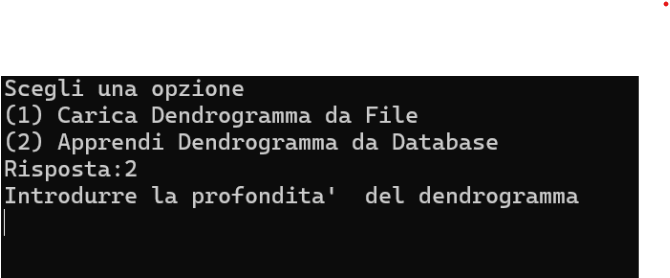
\includegraphics[width=\textwidth]{images/apprendi_datagramma.png}
\end{figure}

Selezionando l'opzione 2, il sistema richiederà l'inserimento del parametro di profondità desiderato per il dendrogramma.

\subsection{Inserimento Profondità}

\begin{figure}[h!]
    \centering
    \includegraphics[width=\textwidth]{images/inserimento_profondità.png}
\end{figure}

Successivamente, l'applicazione proporrà due metodologie di calcolo alternative:
\begin{enumerate}
    \item \textbf{Single-link}: identifica la distanza minima tra cluster, connettendo gli elementi più prossimi tra i gruppi
    \item \textbf{Average-link}: determina la distanza utilizzando la media tra tutti gli elementi dei cluster considerati
\end{enumerate}

\subsubsection{Elaborazione con Single-link}

\begin{figure}[h!]
    \centering
    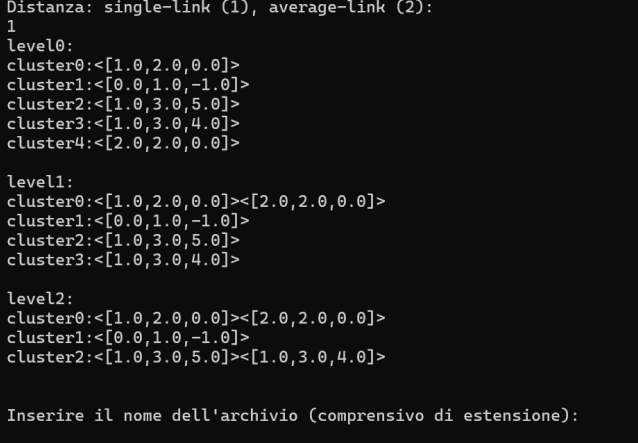
\includegraphics[width=\textwidth]{images/scelta_singleLink.png}
\end{figure}

Selezionando l'opzione Single-link (1), verrà elaborato e visualizzato il dendrogramma risultante. L'applicativo richiederà poi di specificare il nome del file per l'archiviazione del dendrogramma, completo di estensione.

\subsection{Inserimento nome file}

\begin{figure}[h!]
    \centering
    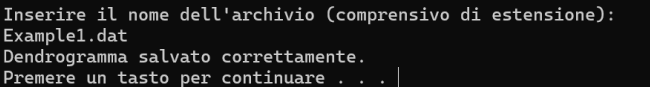
\includegraphics[width=\textwidth]{images/inserimento_nome_file.png}
\end{figure}

Indicare il nome desiderato (esempio: \texttt{Example1.dat}). Il dendrogramma verrà salvato nella cartella \texttt{"saved"} all'interno della directory \texttt{"Jar + Bat"} e l'applicazione terminerà l'esecuzione.

\subsubsection{Elaborazione con Average-link}

\begin{figure}[h!]
    \centering
    \includegraphics[width=\textwidth]{images/scelta_averageLink.png}
\end{figure}

Selezionando l'opzione Average-link (2), il sistema elaborerà il dendrogramma utilizzando il criterio della distanza media e lo visualizzerà a schermo. Successivamente, verrà richiesto di specificare il nome del file per la memorizzazione del dendrogramma, completo di estensione.

\subsection{Percorso operativo - Opzione 1 (Caricamento dendrogramma esistente)}
\begin{figure}[h!]
    \centering
    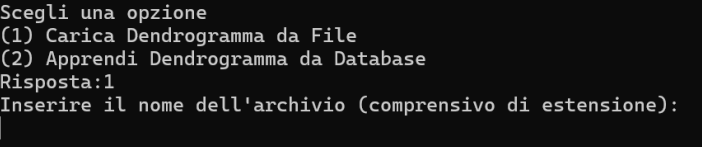
\includegraphics[width=\textwidth]{images/carica_dendrogramma_file.png}
\end{figure}

Selezionando l'opzione 1 per importare un dendrogramma preesistente, sarà necessario indicare il nome completo del file archivio, comprensivo di estensione. I file precedentemente salvati sono localizzati nella cartella \texttt{"saved"} all'interno della directory \texttt{"Jar + Bat"}.

\subsection{Inserimento nome archivio con estensione}

\begin{figure}[h!]
    \centering
    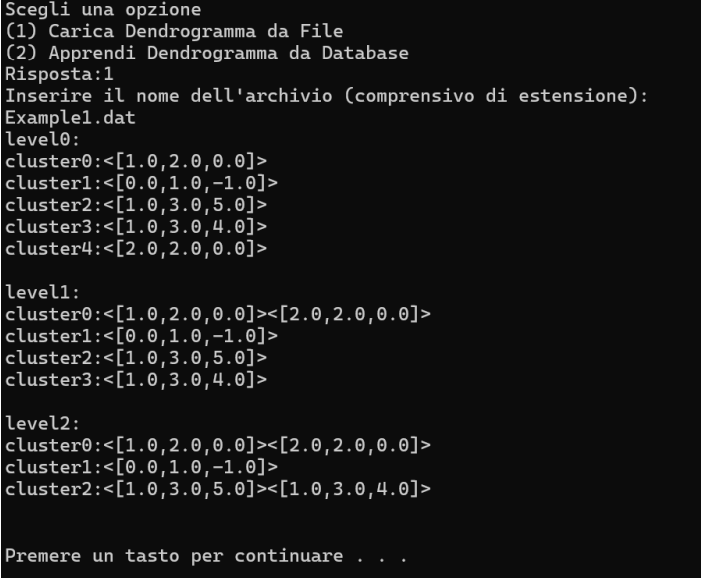
\includegraphics[width=\textwidth]{images/inserimento_nome_archivio.png}
\end{figure}

Dopo l'inserimento del nome dell'archivio, il sistema visualizzerà il dendrogramma caricato e concluderà l'esecuzione.

\section{TEST A-CLUS BASE}

Durante la fase di testing, sono stati analizzati diversi scenari critici per validare la robustezza dell'applicazione:

\substection{Gestione di tabelle inesistenti}

\begin{figure}[h!]
    \centering
    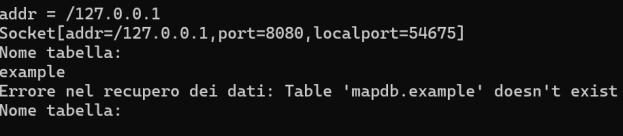
\includegraphics[width=\textwidth]{images/errore_tabella.png.png}
\end{figure}

Quando viene specificato un identificativo di tabella non presente nel database, il sistema visualizza un appropriato messaggio diagnostico e offre all'utente la possibilità di inserire una denominazione alternativa.


\subsection{Validazione delle selezioni di menù}

\begin{figure}[h!]
    \centering
    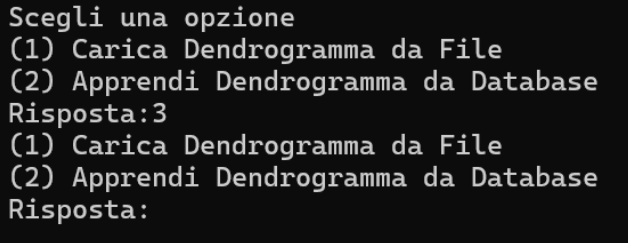
\includegraphics[width=\textwidth]{images/errore_men.png}
\end{figure}

L'inserimento di valori non conformi alle opzioni disponibili (diversi da 1 o 2) viene intercettato, consentendo all'utente di ripetere la selezione senza interruzioni del flusso operativo.

\subsubsection{Controllo sull'esistenza degli archivi} 
\begin{figure}[h!]
    \centering
    \includegraphics[width=\textwidth]{images/controllo_archivi.png}
\end{figure}
Nel caso di caricamento di un dendrogramma precedentemente salvato, il sistema verifica l'esistenza dell'archivio specificato. In caso negativo, viene presentata una notifica e l'applicazione termina la sessione.

\subsubsection{Validazione parametri di profondità} 
    \begin{figure}[h!]
        \centering
        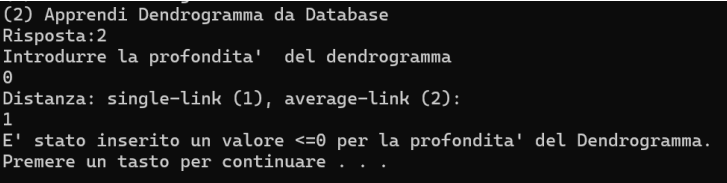
\includegraphics[width=\textwidth]{images/0_valore_errato.png}
    \end{figure}

    \begin{figure}[h!]
        \centering
        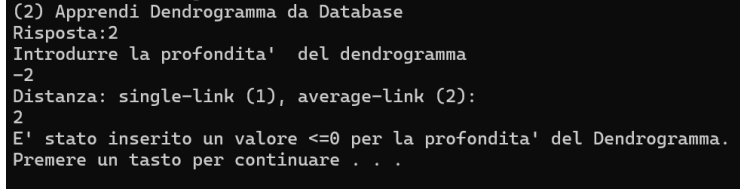
\includegraphics[width=\textwidth]{images/-2_valore_errato.png}
    \end{figure}

    L'inserimento di valori non ammissibili per il parametro di profondità (zero o negativi) viene rilevato dal sistema che, pur proseguendo con la richiesta del metodo di calcolo, interromperà l'elaborazione notificando l'anomalia.

\subsubsection{Controllo selezioni metodologiche} 
    
\begin{figure}[h!]
        \centering
        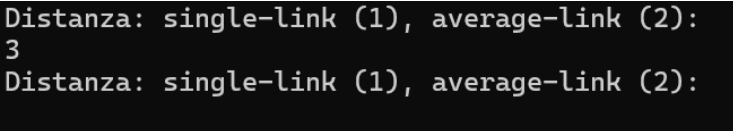
\includegraphics[width=\textwidth]{images/controllo_metodologie.png}
    \end{figure}
    L'inserimento di opzioni non valide per la selezione della metodologia di calcolo delle distanze viene gestito permettendo all'utente di riformulare la propria scelta.

\subsubsection{Verifica di compatibilità dimensionale} 
    \begin{figure}[h!]
        \centering
        \includegraphics[width=\textwidth]{images/compatibilità_dimensionale.png}
    \end{figure}
    Il sistema controlla la congruenza tra la cardinalità degli esempi nella tabella corrente e quella memorizzata nell'oggetto serializzato. In caso di incongruenza, viene visualizzato un messaggio esplicativo e l'esecuzione viene terminata.

\subsection{Gestione connettività client-server}
\begin{figure}[h!]
    \centering
    \includegraphics[width=\textwidth]{images/connettività_clientserver.png.png}
\end{figure}
L'avvio del client in assenza del componente server attivo genera un tentativo di connessione all'indirizzo locale (127.0.0.1) che, non trovando un endpoint disponibile, risulta in un rifiuto della connessione con relativa notifica.

\subsubsection{Elaborazione su dataset vuoti} 
    \begin{figure}[h!]
        \centering
        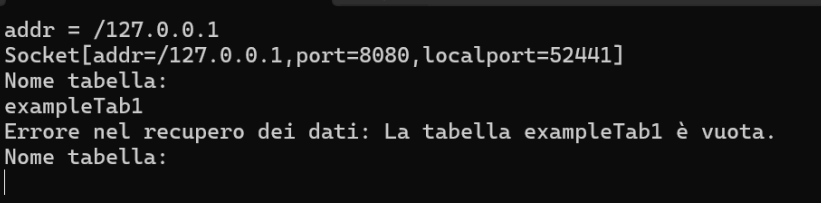
\includegraphics[width=\textwidth]{images/dataset_vuoti.png}
    \end{figure}

Quando l'utente tenta di eseguire un'analisi di clustering su una tabella priva di contenuti, il sistema identifica la condizione e fornisce un'appropriata segnalazione.


\section{Cambiamenti}

\subsection{Cambiamenti Motivati nella Versione Base Rispetto i Requisiti del Progetto}

\begin{enumerate}
    \item \textbf{Metodo getLength() in ClusterSet / Metodo getLevel0Length() in HierarchicalClusterMiner:}
    \begin{itemize}
        \item \textbf{Descrizione getLength():} Questo metodo restituisce la lunghezza dell'array C in ClusterSet.
        \item \textbf{Descrizione getLevel0Length():} Questo metodo restituisce la lunghezza del set di cluster al livello 0 del dendrogramma.
        \item \textbf{Motivazione:} Abbiamo aggiunto questi metodi per ottenere il numero di elementi presenti nel ClusterSet al livello 0 del dendrogramma e per passare tale informazione al metodo loadDendrogramFromFile() in ServerOneClient. Questo permette di verificare qui che il numero di esempi nella tabella scelta non sia minore del numero di esempi con cui è stato salvato il dendrogramma precedentemente.
    \end{itemize}
    
    \item \textbf{Metodo getDepth() in HierarchicalClusterMiner:}
    \begin{itemize}
        \item \textbf{Descrizione getDepth():} Questo metodo restituisce la profondità del dendrogramma in HierarchicalClusterMiner.
        \item \textbf{Motivazione:} Abbiamo aggiunto questo metodo per verificare nel metodo loadDendrogramFromFile() in ServerOneClient che la profondità del dendrogramma caricato da file non sia maggiore del numero di esempi nella tabella scelta dall'utente.
    \end{itemize}
\end{enumerate}

\subsection{Cambiamenti Motivati nella Versione Estesa Rispetto alla Base}

\begin{enumerate}
    \item \textbf{Rimossa responsabilità gestione macchina a stati nel server.}\\
    Nella versione base del programma, il metodo run di ServerOneClient memorizzava l'oggetto Data, che rappresentava la tabella contenente il dataset scelto dall'utente. Questo oggetto era creato alla prima richiesta dal client, nel momento in cui l'utente specificava quale tabella del database utilizzare. I dati erano poi conservati all'interno del thread avviato per ciascuna connessione tra client e server, e mantenuti attivi grazie a un ciclo while true, che proseguiva fino alla disconnessione del client.
    
    Nella versione estesa, invece, il client gestisce gli aggiornamenti (Updates) inviati dall'API di Telegram, che contengono i messaggi degli utenti diretti al bot. Teoricamente, il server della versione base potrebbe essere compatibile con il client della versione estesa, poiché è progettato per gestire connessioni multiple tramite multithreading: ogni aggiornamento del bot potrebbe quindi attivare un thread separato del server, avviando una nuova connessione Socket.
    
    Tuttavia, questa soluzione è adatta solo se la connessione socket può rimanere aperta a lungo. Se, per esempio, un utente inviasse un messaggio ora e il successivo solo una settimana dopo, mantenere la connessione aperta risulterebbe inefficiente e costoso, poiché l'unico scopo sarebbe mantenere vivo l'oggetto Data nel thread.
    
    Per questa ragione e per garantire al server una struttura generica, capace di interfacciarsi con client di natura diversa, abbiamo deciso di spostare l'oggetto Data nel client esteso, insieme ad altre informazioni necessarie per la gestione degli stati. Ad esempio, in futuro potrebbero esistere sia un client web sia un client bot Telegram. Supponiamo che un utente esegua due clustering uno sulla versione web e una sulla versione bot Telegram; mantenere tutti i dati di stato sul server limiterebbe la possibilità di separare l'interazione su dispositivi diversi, oltre a imporre uno schema fisso basato sulla macchina a stati anche per i client che non lo necessitano. Un client senza macchina a stati potrebbe, ad esempio, essere una versione web in cui le operazioni ``Carica tabella'', ``Profondità'', ``Distanza'' e ``Clustering'' sono eseguite in un'unica richiesta, senza passare attraverso stati successivi.
    
    Nel nuovo client quando riceve un aggiornamento da parte di un nuovo utente, crea un record nel dizionario memorizzando come chiave l'ID Telegram dell'utente e come valore un'istanza della classe StateContext, che gestisce la macchina a stati. Quando un utente invia un messaggio e la sua chiave è già presente nel dizionario, il sistema esegue le operazioni sul StateContext già esistente per quell'utente. StateContext è responsabile della gestione della macchina a stati e contiene uno Stack di stati, che memorizza la cronologia degli stati attraversati dall'utente, più l'ultimo stato attivo in cui applicare gli aggiornamenti. Inoltre, StateContext include una classe Dati che funge da aggregatore di vari dati condivisi tra gli stati e include anche l'oggetto Data (dataset) originale della versione base del server. In questo modo, il sistema può gestire la persistenza e la transizione degli stati per ciascun utente, senza dover mantenere una connessione server-client attiva per tempi prolungati.
    
    La classe StateContext contiene i seguenti attributi di istanza:
    \begin{itemize}
        \item \textbf{Stack<State> StateHistory:} rappresenta la cronologia degli stati attraversati dall'utente. Di default, lo stack contiene lo stato iniziale passato nel costruttore e viene poi popolato aggiungendo ogni nuovo stato tramite operazioni di push. Questo approccio facilita il rollback degli stati. Ad esempio, se l'utente è nello stato 3 e lo stack contiene gli stati [3, 2, 1], un rollback eseguirà un pop dello stato 3, riportando automaticamente l'utente allo stato 2, senza la necessità di gestire manualmente ogni singolo caso di retrocessione.
    \end{itemize}
    
    Ogni stato ha la proprietà allowBack. Se impostata su false (valore di default), consente il rollback dallo stato corrente. Se invece è impostata su true, non è possibile tornare indietro da quello stato. Questo comportamento è stato applicato allo stato iniziale, poiché non è consentito fare rollback una volta entrati nello stato di avvio. Ad esempio, gli stati Clustering e ShowSavedClustering offrono opzioni per tornare allo stato principale (ossia Start), ma una volta raggiunto lo stato Start, il rollback non è consentito poiché segna l'inizio di una nuova iterazione.
    
    Ogni stato è suddiviso in due fasi di operazione:
    \begin{itemize}
        \item \textbf{Pre-Operation:} viene eseguita una sola volta quando lo stato viene creato o resettato. Nel flusso di lavoro attuale, ogni stato fornisce all'utente una serie di operazioni da eseguire, attende la risposta dell'utente e la valida. La fase di preOperation corrisponde all'operazione di chiedere all'utente cosa desidera fare.
        \item \textbf{Post-Operation:} valida la risposta dell'utente e gestisce le transizioni verso altri stati. Passando StateContext come parametro al metodo postOperation, è possibile richiamare il metodo changeState per indicare il nuovo stato da eseguire. Una volta cambiato lo stato, viene eseguita automaticamente la preOperation del nuovo stato, permettendo al sistema di rispondere immediatamente all'utente con il nuovo set di operazioni disponibili per quello stato.
    \end{itemize}
    
    Durante l'esecuzione di una delle due operazioni possono verificarsi errori dovuti a input non validi, dati incorretti o problemi nelle risposte socket. Il comportamento in caso di errore varia in base alla fase dell'operazione:
    \begin{itemize}
        \item \textbf{Pre-Operation:} un errore in questa fase causa un rollback automatico allo stato precedente. Ad esempio, nella fase di pre-operazione del Clustering, può verificarsi un errore se l'utente sceglie un nome per il file di salvataggio del clustering che esiste già dallo stato precedente. In tal caso, il blocco catch esegue un rollback allo stato precedente (con apposito log d'errore), ovvero lo stato ChooseName della post-operazione, permettendo all'utente di inserire un nuovo nome per il file di salvataggio.
        \item \textbf{Post-Operation:} in questa fase, un eventuale errore non altera il flusso del programma, ma comporta la ripetizione della post-operazione. Ad esempio, nel metodo ChooseDepth, la post-operazione convalida la profondità scelta dall'utente; se questa profondità non è valida o fuori range, viene generata un'eccezione che porta al riavvio della post-operazione (con apposito log d'errore), consentendo all'utente di inserire una nuova profondità valida.
    \end{itemize}
\end{enumerate}

\end{document}

\section{Eseguire A-CLus Esteso}


Per avviare la versione estesa del progetto A-CLus, è necessario seguire i seguenti passaggi:
\begin{enumerate}
    \item Accedere alla directory \texttt{H-CLUS\_Esteso/Jar + Bat}
    \item All'interno della suddetta cartella, eseguire il file \texttt{Start Server.bat} con doppio click, mantenendo attiva la finestra del prompt dei comandi
    \item Procedere con l'avvio del file \texttt{Start Client.bat} tramite doppio click, il quale genererà un'ulteriore finestra di comando
    \item Aprire Telegram e cercare "A-Clus" utilizzando il tag "@A\_Clus\_bot" oppure cliccando sul \href{https://shorturl.at/r07hj}{link diretto}
\end{enumerate}

\begin{tcolorbox}[colback=white, colframe=gray, title=Avvertenza]
    È necessario mantenere attivi i terminali del server e del client per garantire la comunicazione tra tutte le componenti del sistema.
\end{tcolorbox}

\subsection{Avvio dall'ambiente di sviluppo}

La procedura di avvio del progetto A-CLus può essere eseguita anche direttamente dall'ambiente di sviluppo, in maniera analoga alla versione base. 

\begin{enumerate}
    \item Aprire il progetto \texttt{A-CLus\_Esteso}
    \item Eseguire il file \texttt{MultiServer.java} presente nella cartella \texttt{server/src/server} per avviare il server
    \item Eseguire il file \texttt{Main.java} presente nella cartella \texttt{client/src/client} per avviare il client
    \item Aprire Telegram e cercare "A-Clus" utilizzando il tag "@A\_Clus\_bot" oppure cliccando sul \href{https://shorturl.at/r07hj}{link diretto} per accedere al bot 
\end{enumerate}




\section{Cambiamenti}

\subsection{Cambiamenti Motivati nella Versione Base Rispetto i Requisiti del Progetto}

\begin{enumerate}
    \item \textbf{Metodo getLength() in ClusterSet / Metodo getLevel0Length() in HierarchicalClusterMiner:}
    \begin{itemize}
        \item \textbf{Descrizione getLength():} Questo metodo restituisce la lunghezza dell'array C in ClusterSet.
        \item \textbf{Descrizione getLevel0Length():} Questo metodo restituisce la lunghezza del set di cluster al livello 0 del dendrogramma.
        \item \textbf{Motivazione:} Abbiamo aggiunto questi metodi per ottenere il numero di elementi presenti nel ClusterSet al livello 0 del dendrogramma e per passare tale informazione al metodo loadDendrogramFromFile() in ServerOneClient. Questo permette di verificare qui che il numero di esempi nella tabella scelta non sia minore del numero di esempi con cui è stato salvato il dendrogramma precedentemente.
    \end{itemize}
    
    \item \textbf{Metodo getDepth() in HierarchicalClusterMiner:}
    \begin{itemize}
        \item \textbf{Descrizione getDepth():} Questo metodo restituisce la profondità del dendrogramma in HierarchicalClusterMiner.
        \item \textbf{Motivazione:} Abbiamo aggiunto questo metodo per verificare nel metodo loadDendrogramFromFile() in ServerOneClient che la profondità del dendrogramma caricato da file non sia maggiore del numero di esempi nella tabella scelta dall'utente.
    \end{itemize}
\end{enumerate}

\subsection{Cambiamenti Motivati nella Versione Estesa Rispetto alla Base}

\begin{enumerate}
    \item \textbf{Rimossa responsabilità gestione macchina a stati nel server.}\\
    Nella versione base del programma, il metodo run di ServerOneClient memorizzava l'oggetto Data, che rappresentava la tabella contenente il dataset scelto dall'utente. Questo oggetto era creato alla prima richiesta dal client, nel momento in cui l'utente specificava quale tabella del database utilizzare. I dati erano poi conservati all'interno del thread avviato per ciascuna connessione tra client e server, e mantenuti attivi grazie a un ciclo while true, che proseguiva fino alla disconnessione del client.
    
    Nella versione estesa, invece, il client gestisce gli aggiornamenti (Updates) inviati dall'API di Telegram, che contengono i messaggi degli utenti diretti al bot. Teoricamente, il server della versione base potrebbe essere compatibile con il client della versione estesa, poiché è progettato per gestire connessioni multiple tramite multithreading: ogni aggiornamento del bot potrebbe quindi attivare un thread separato del server, avviando una nuova connessione Socket.
    
    Tuttavia, questa soluzione è adatta solo se la connessione socket può rimanere aperta a lungo. Se, per esempio, un utente inviasse un messaggio ora e il successivo solo una settimana dopo, mantenere la connessione aperta risulterebbe inefficiente e costoso, poiché l'unico scopo sarebbe mantenere vivo l'oggetto Data nel thread.
    
    Per questa ragione e per garantire al server una struttura generica, capace di interfacciarsi con client di natura diversa, abbiamo deciso di spostare l'oggetto Data nel client esteso, insieme ad altre informazioni necessarie per la gestione degli stati. Ad esempio, in futuro potrebbero esistere sia un client web sia un client bot Telegram. Supponiamo che un utente esegua due clustering uno sulla versione web e una sulla versione bot Telegram; mantenere tutti i dati di stato sul server limiterebbe la possibilità di separare l'interazione su dispositivi diversi, oltre a imporre uno schema fisso basato sulla macchina a stati anche per i client che non lo necessitano. Un client senza macchina a stati potrebbe, ad esempio, essere una versione web in cui le operazioni ``Carica tabella'', ``Profondità'', ``Distanza'' e ``Clustering'' sono eseguite in un'unica richiesta, senza passare attraverso stati successivi.
    
    Nel nuovo client quando riceve un aggiornamento da parte di un nuovo utente, crea un record nel dizionario memorizzando come chiave l'ID Telegram dell'utente e come valore un'istanza della classe StateContext, che gestisce la macchina a stati. Quando un utente invia un messaggio e la sua chiave è già presente nel dizionario, il sistema esegue le operazioni sul StateContext già esistente per quell'utente. StateContext è responsabile della gestione della macchina a stati e contiene uno Stack di stati, che memorizza la cronologia degli stati attraversati dall'utente, più l'ultimo stato attivo in cui applicare gli aggiornamenti. Inoltre, StateContext include una classe Dati che funge da aggregatore di vari dati condivisi tra gli stati e include anche l'oggetto Data (dataset) originale della versione base del server. In questo modo, il sistema può gestire la persistenza e la transizione degli stati per ciascun utente, senza dover mantenere una connessione server-client attiva per tempi prolungati.
    
    La classe StateContext contiene i seguenti attributi di istanza:
    \begin{itemize}
        \item \textbf{Stack <State> StateHistory:} rappresenta la cronologia degli stati attraversati dall'utente. Di default, lo stack contiene lo stato iniziale passato nel costruttore e viene poi popolato aggiungendo ogni nuovo stato tramite operazioni di push. Questo approccio facilita il rollback degli stati. Ad esempio, se l'utente è nello stato 3 e lo stack contiene gli stati [3, 2, 1], un rollback eseguirà un pop dello stato 3, riportando automaticamente l'utente allo stato 2, senza la necessità di gestire manualmente ogni singolo caso di retrocessione.
    \end{itemize}
    
    Ogni stato ha la proprietà allowBack. Se impostata su false (valore di default), consente il rollback dallo stato corrente. Se invece è impostata su true, non è possibile tornare indietro da quello stato. Questo comportamento è stato applicato allo stato iniziale, poiché non è consentito fare rollback una volta entrati nello stato di avvio. Ad esempio, gli stati Clustering e ShowSavedClustering offrono opzioni per tornare allo stato principale (ossia Start), ma una volta raggiunto lo stato Start, il rollback non è consentito poiché segna l'inizio di una nuova iterazione.
    
    Ogni stato è suddiviso in due fasi di operazione:
    \begin{itemize}
        \item \textbf{Pre-Operation:} viene eseguita una sola volta quando lo stato viene creato o resettato. Nel flusso di lavoro attuale, ogni stato fornisce all'utente una serie di operazioni da eseguire, attende la risposta dell'utente e la valida. La fase di preOperation corrisponde all'operazione di chiedere all'utente cosa desidera fare.
        \item \textbf{Post-Operation:} valida la risposta dell'utente e gestisce le transizioni verso altri stati. Passando StateContext come parametro al metodo postOperation, è possibile richiamare il metodo changeState per indicare il nuovo stato da eseguire. Una volta cambiato lo stato, viene eseguita automaticamente la preOperation del nuovo stato, permettendo al sistema di rispondere immediatamente all'utente con il nuovo set di operazioni disponibili per quello stato.
    \end{itemize}
    
    Durante l'esecuzione di una delle due operazioni possono verificarsi errori dovuti a input non validi, dati incorretti o problemi nelle risposte socket. Il comportamento in caso di errore varia in base alla fase dell'operazione:
    \begin{itemize}
        \item \textbf{Pre-Operation:} un errore in questa fase causa un rollback automatico allo stato precedente. Ad esempio, nella fase di pre-operazione del Clustering, può verificarsi un errore se l'utente sceglie un nome per il file di salvataggio del clustering che esiste già dallo stato precedente. In tal caso, il blocco catch esegue un rollback allo stato precedente (con apposito log d'errore), ovvero lo stato ChooseName della post-operazione, permettendo all'utente di inserire un nuovo nome per il file di salvataggio.
        \item \textbf{Post-Operation:} in questa fase, un eventuale errore non altera il flusso del programma, ma comporta la ripetizione della post-operazione. Ad esempio, nel metodo ChooseDepth, la post-operazione convalida la profondità scelta dall'utente; se questa profondità non è valida o fuori range, viene generata un'eccezione che porta al riavvio della post-operazione (con apposito log d'errore), consentendo all'utente di inserire una nuova profondità valida.
    \end{itemize}
\end{enumerate}


\section{Macchina a stati}

\begin{figure}[h!]
    \centering
    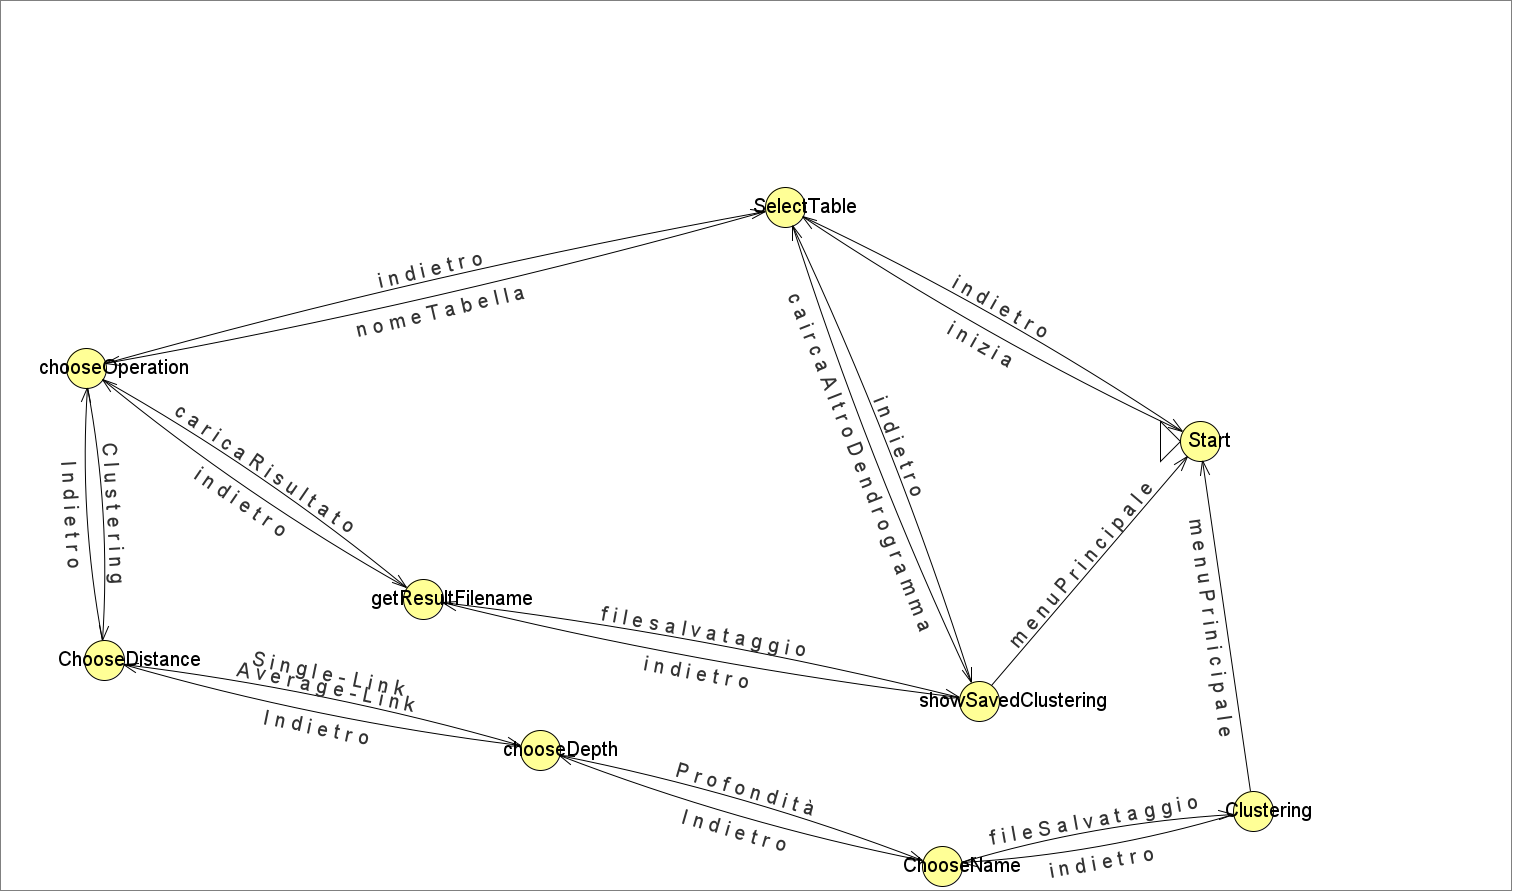
\includegraphics[width=\textwidth]{images/macchina a stati.png}
    \caption{Macchina a stati del bot Telegram}
\end{figure}

\end{document}